\section{Model and open loop analysis}
\subsection{Model analysis}
The continuous state space model where $u=V$ (voltage on the motor) and x=$[\theta \ \alpha \  \dot{\theta} \ \dot{\alpha} ]$ is theoretical derived in the assignment and leads to the following system. The system can only directly measure $\theta$ and $\alpha$, so these determine the matrix C and D.

$$
\begin{cases}
\dot{x}=Ax+Bu \\
y=Cx+Du
\end{cases}
$$

$$
A=
\begin{bmatrix}
0 & 0 & 1 & 0 \\
0 & 0 & 0 & 1 \\
0 & 40.7 & -12.2 & 0 \\
0 & 38.6 & -4.7 & 0 
\end{bmatrix}
B=
\begin{bmatrix}
0 \\
0 \\
23.3 \\
8.3
\end{bmatrix}
C=
\begin{bmatrix}
1 & 0 & 0 & 0\\
0 & 1 & 0 & 0
\end{bmatrix}
D=
\begin{bmatrix}
0 & 0
\end{bmatrix}
$$

\subsection{Open loop analysis}

The system contains 1 unstable pole at about 5.3 (see figure~\ref{fig:zplot system}), this obviously means that the system is unstable. The rank of the controllability matrix is 4, the smallest singular value of the controllability matrix is 1.7. So the system is controllable, controllability is necessary if you want to control a system. The observability matrix is of rank 4 which with a smallest singular value of 1. So the system is observable. If a system is observable and controllable than it is also the minimal realisation of the system. This means the system with the minimal numbers of states possible that fits the given behaviour. If the system is controllable then it's stabilizable and if its observable then it's also detectable which means that if there are unstable states, they you can at least detect unstability.

\begin{figure}[H]
	\centering
	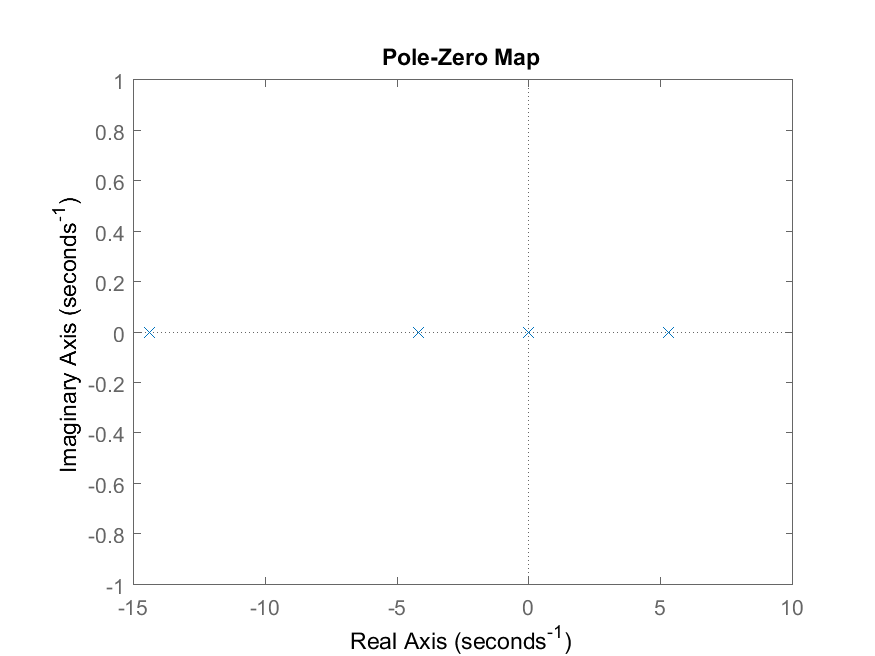
\includegraphics[width=0.5\textwidth]{./part1_analysis/zplot.png}
	\caption{plot of poles and zeros}
	\label{fig:zplot system}
\end{figure}

\subsection{Control goals}
When designing a controller tradeoffs have to be made.If it would be possible to create a fast,robust,.. controller then this would be the best option. However in this report robustness was preferred over speed. However the robustness comes at a price, if robustness is preferred then the controller will lose speed. 

So the first priority when designing this controller was to make a stable system. After stabilization is reached, we want the system to be rather robust, it should not be very fast as this will result in a nervous system. We would like that the system can track setpoints up to some step-responses. But our objective is more a robustness system than a fast one.

%One of the most forward ways to check if the controller wasn't to nervous was to listen to the sound of the device. A nervous controller will react very fast on small changes and this creates a very unhealthy clicking noise. This obviously cant be good for the mechanical components. 
% M: Mechanical and electrical.
